\begin{figure}[H]
    \renewcommand{\figurename}{Рисунок}
    \centering{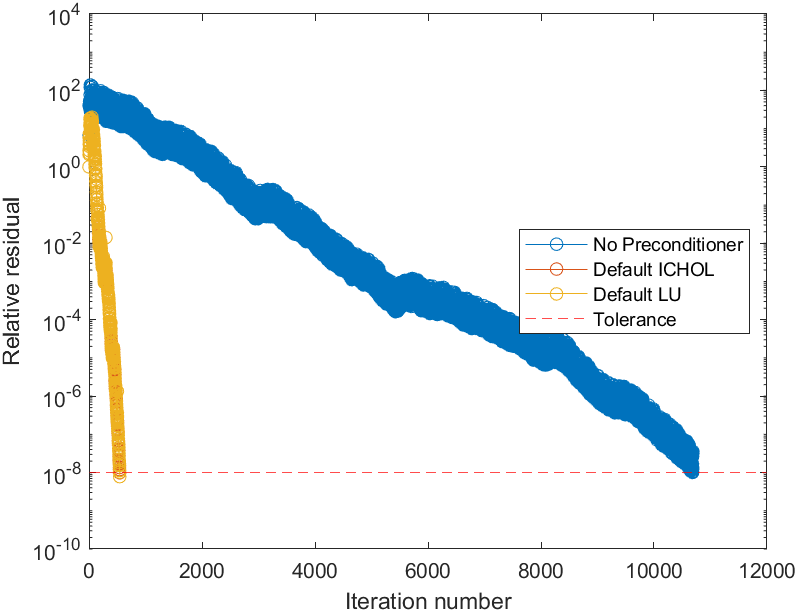
\includegraphics[scale=0.70]{img/G2/bicg}}
    \caption{История невязок методом bicg для матрицы G2\_circuit}
    \label{fig:image_44}
\end{figure}

\begin{figure}[H]
    \renewcommand{\figurename}{Рисунок}
    \centering{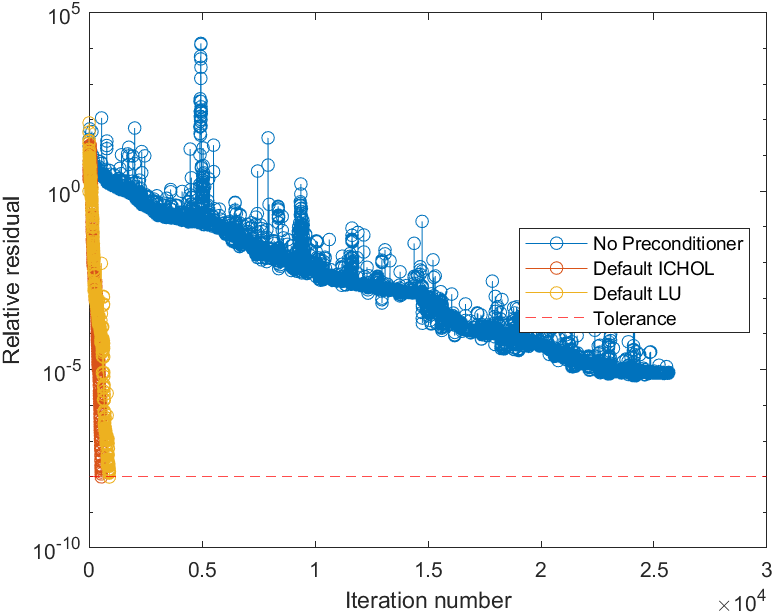
\includegraphics[scale=0.70]{img/G2/bicgstab}}
    \caption{История невязок методом bicgstab для матрицы G2\_circuit}
    \label{fig:image_45}
\end{figure}

\begin{figure}[H]
    \renewcommand{\figurename}{Рисунок}
    \centering{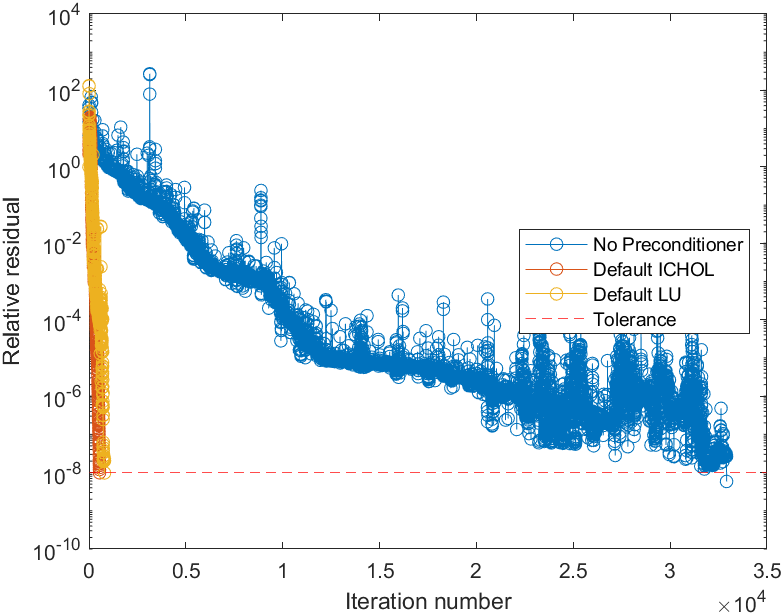
\includegraphics[scale=0.70]{img/G2/bicgstabl}}
    \caption{История невязок методом bicgstabl для матрицы G2\_circuit}
    \label{fig:image_46}
\end{figure}

\begin{figure}[H]
    \renewcommand{\figurename}{Рисунок}
    \centering{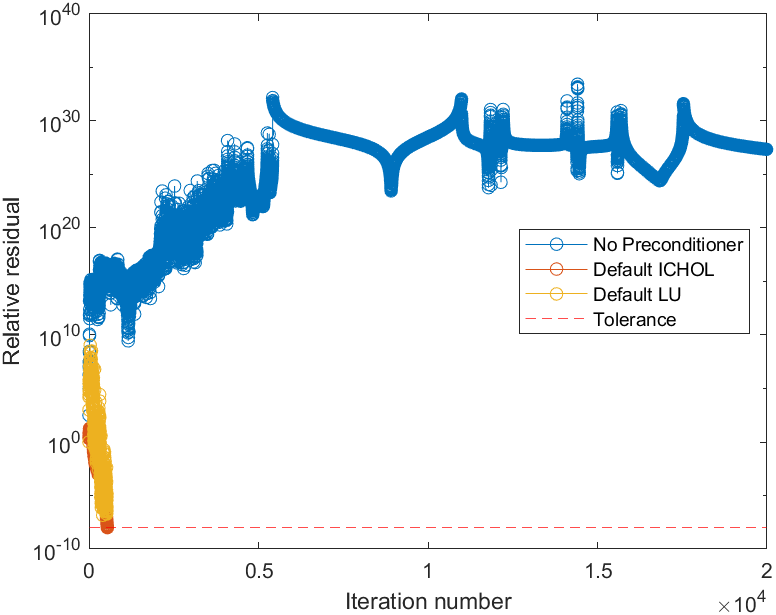
\includegraphics[scale=0.70]{img/G2/cgs}}
    \caption{История невязок методом cgs для матрицы G2\_circuit}
    \label{fig:image_47}
\end{figure}

\begin{figure}[H]
    \renewcommand{\figurename}{Рисунок}
    \centering{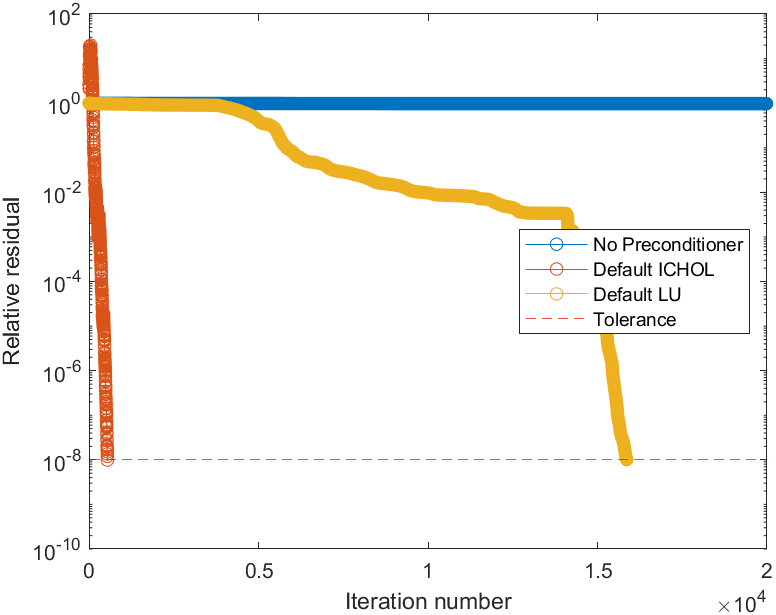
\includegraphics[scale=0.70]{img/G2/lsqr}}
    \caption{История невязок методом lsqr для матрицы G2\_circuit}
    \label{fig:image_48}
\end{figure}

\begin{figure}[H]
    \renewcommand{\figurename}{Рисунок}
    \centering{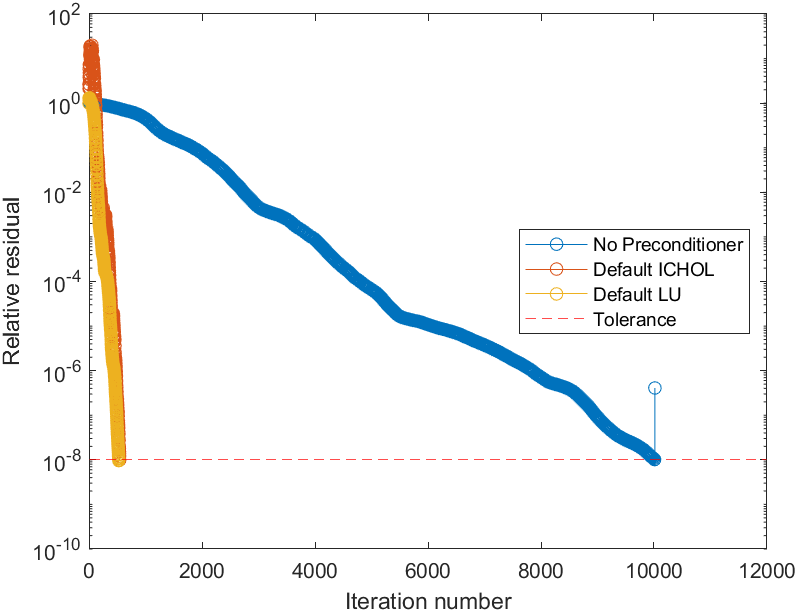
\includegraphics[scale=0.70]{img/G2/minres}}
    \caption{История невязок методом minres для матрицы G2\_circuit}
    \label{fig:image_49}
\end{figure}

\begin{figure}[H]
    \renewcommand{\figurename}{Рисунок}
    \centering{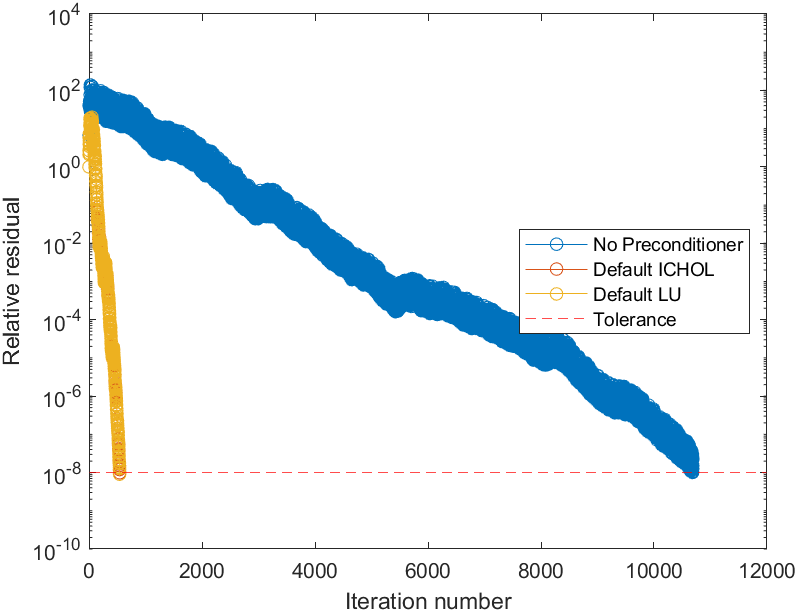
\includegraphics[scale=0.70]{img/G2/pcg}}
    \caption{История невязок методом pcg для матрицы G2\_circuit}
    \label{fig:image_50}
\end{figure}

\begin{figure}[H]
    \renewcommand{\figurename}{Рисунок}
    \centering{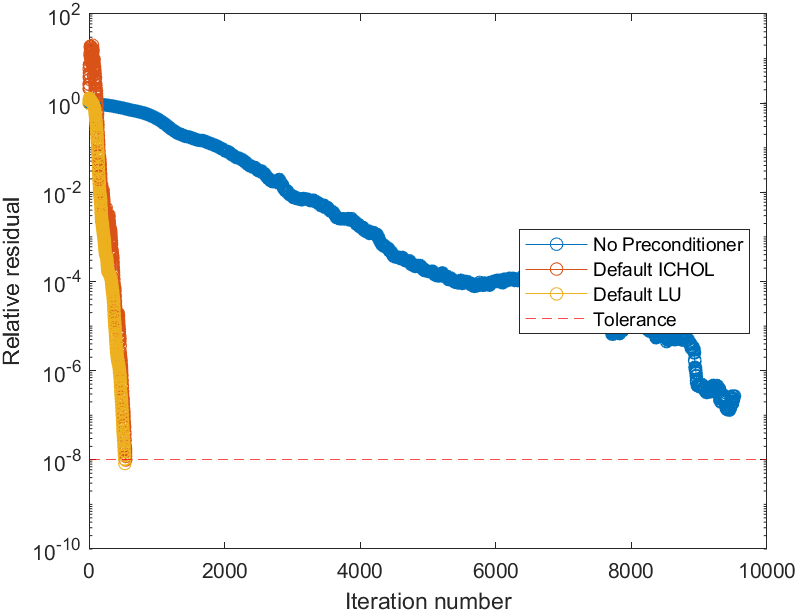
\includegraphics[scale=0.70]{img/G2/qmr}}
    \caption{История невязок методом qmr для матрицы G2\_circuit}
    \label{fig:image_51}
\end{figure}

\begin{figure}[H]
    \renewcommand{\figurename}{Рисунок}
    \centering{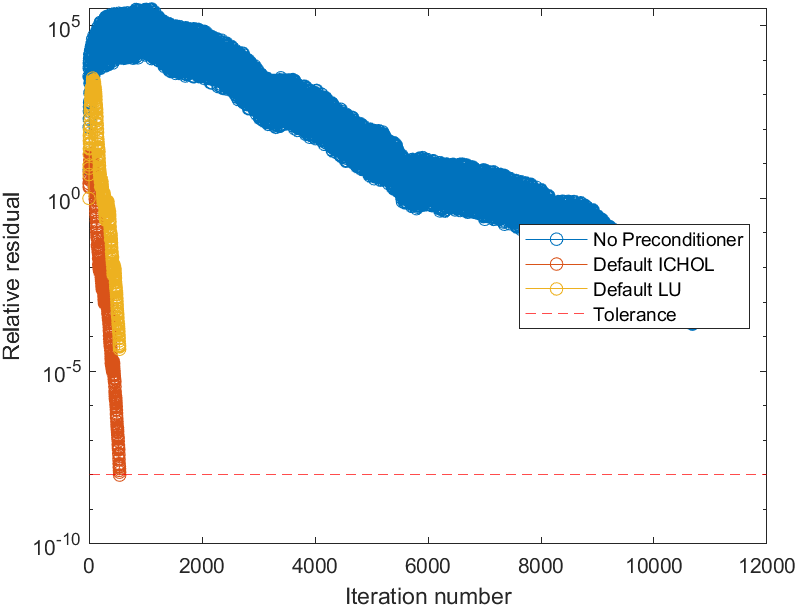
\includegraphics[scale=0.70]{img/G2/symmlq}}
    \caption{История невязок методом symmlq для матрицы G2\_circuit}
    \label{fig:image_52}
\end{figure}

\begin{figure}[H]
    \renewcommand{\figurename}{Рисунок}
    \centering{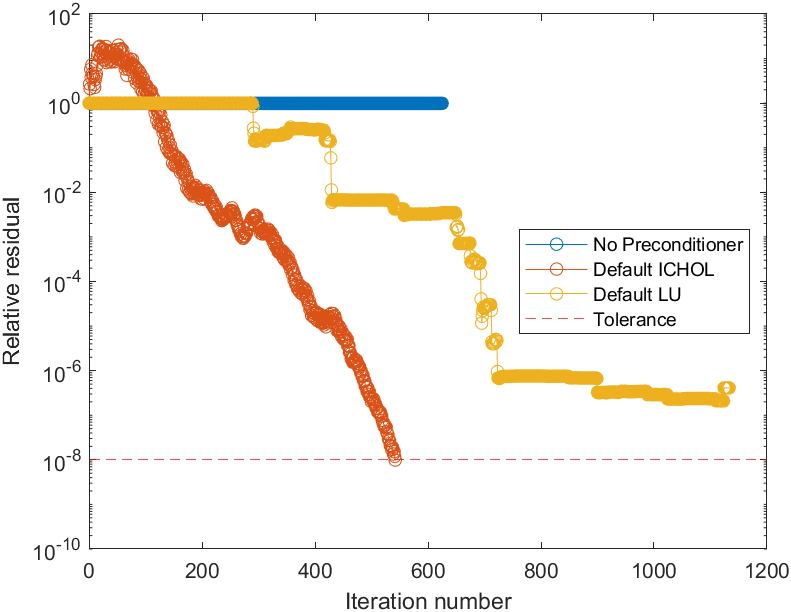
\includegraphics[scale=0.70]{img/G2/tfqmr}}
    \caption{История невязок методом tfqmr для матрицы G2\_circuit}
    \label{fig:image_53}
\end{figure}
